\label{ch:project}

Projekt składa się z~kilku współpracujących ze sobą modułów, posiadających odrębne role. Każdy z~nich wykonano osobno, a~następie połączono --- pośrednio lub bezpośrednio --- w~jeden, działający system.

Pierwszym elementem jest fizyczny pojazd, na który składa się układ elektroniczny i~wydrukowany model 3D. Jest on elementem centralnym, wokół którego budowana jest reszta systemu.

Drugim elementem jest aplikacja mobilna na system Android. Jej zadaniem jest wysyłanie do pojazdu informacji o~nowym pomiarze, jego rozpoczęcie oraz zakończenie.

Trzeci element to skrypt w~języku Python. Odbiera on z~pojazdu dane pomiarowe i~zapisuje je do pliku .csv celem dalszej pracy na uzyskanych danych.

Ostatni element to skrypt w~języku MATLAB. Odczytuje on zapisane poprzednio dane z pliku .csv i~przetwarza je w celu prezentacji.

\section{Pojazd}
Projekt pojazdu zakłada 4 koła, z czego 2 przednie na wspólnej osi skrętnej, a 2 tylne na osi statycznej obrotowej zasilane silnikami DC. W pojeździe muszą znajdować się sloty na akumulatory zasilające, przestrzeń na układ elektroniczny z przewodami, oraz musi zostać zapewniony sposób stabilnego montażu silników, tak by zminimalizować wpływ zakłóceń pomiarowych spowodowanych przez drgania i przemieszczanie się osi w trakcie działania układu.

\subsection*{Druk 3D}
Technologia druku 3D opiera się na nakładaniu na siebie kolejnych, cienkich warstw stopionego materiału. Jest to metoda addytywna obróbki materiału. Dwie główne technologie druku to FDM (ang. \english{Fused Deposition Modeling}) oraz DLP (ang.~\english{Digital Light Processing}), w których stosuje się odpowiednio plastiki lub żywice\cite{bib:pracakrzysztofaserafina}. Drukarka SV06 umożliwia druk w technologii FDM, zdecydowano więc na użycie najpopularniejszego plastiku typu PLA \english{Polylactic Acid}.

Przed przystąpieniem do projektu, należy rozważyć założenia w kontekście ograniczeń i możlilwości zastosowanej technologii. Pierwszym ograniczeniem jest wymiar druku. Głowica podająca materiał może w~zależności od konfiguracji drukarki poruszać się w~różny sposób. 3~podstawowe modele to kartezjański XZ, CoreXY i~delta. Pierwszy z~wymienionych, a~równocześnie najpopularniejszy, wykorzystany został w~zastosowanej drukarce SV06. Ruch głowicy polega w~nim na przemieszczaniu po standardowych współrzędnych kratezjańskich, $x$,~$y$, oraz~$z$. Wynika z~tego ograniczona wielkość drukowanych modeli --- zasięg drukarki jest limitowany. Model SV06 posiada przestrzeń druku w~kształcie sześcianu o~krawędzi 220~mm. W~praktyce, dla bezpieczeństwa drukarki jak i~samego druku, odejmuje się pewien margines od każdej krawędzi. Najczęściej jest to około 5~mm z~każdej strony w każdym wymiarze, co w~przypadku 220~mm ustawia efektywny bezpieczny wymiar druku na 210~mm, dając sześcian o krawędzi 210~mm.

Wiadomo więc, że maksymalny (bezpieczny) rozmiar pojazdu to 210$x$210$x$210~mm. Minimalny wymiar nie jest narzucony odgórnie przez technologię lub założenia, lecz pośrednio przez konieczność ograniczenia masy pojazdu ze względu na skończoną ilość mocy silników. Model pojazdu powinien być więc mniejszy niż maksymalny wymiar, i~jednocześnie możliwie jak najmniejszy. Drogą eksperymentalną wyznaczono minimalną grubość ścianek pojazdu, które nie poddają się łatwo zgięciu i~zachowują wysoką sztywność, na 3~mm.

Uwzględnić należy również modułowość pojazdu, wynikającą z~założeń. Moduły pojazdu są 2 --- pierwszy to sama rama pojazdu, drugi to osłona silników determinująca średnicę kół. Początkowo zakładano stworzenie dodatkowych 2 modułów ---- pokrycia wierzchniego, oraz przedniej klapy pojazdu. Nie są one wymagane do prawidłowego działania, jednak dodałyby walorów estetycznych ukrywając elementy wewnętrzne. Z tą myślą projektowano model, zostawiając punkty zaczepowe dla odpowiednich modułów. Pomysł został jednak porzucony ze względu na ograniczony czas.

Pierwsza wersja modelu zakładała szerokość 80~mm i~długość 120~mm. W~trakcie projektowania bardzo szybko stało się jasne, że konieczne będzie pójście na ustępstwa. Pierwszym ustępstwem było porzucenie idei 4~kół. Założenie obiecujące pod kątem wizualnym, lecz w~praktyce wymagające zamontowania dodatkowej osi z~przodu pojazdu wraz z~silnikiem skrętnym, co niepotrzebnie komplikowało projekt. W~związku z~porzuceniem kół przednich o~wspólnej, skrętnej osi, konieczne stało się zastosowanie rozwiązania zastępczego. Wybór padł na pojedyncze obrotowe koło podporowe. Drugim ustępstwem była długość i~szerokość. Zastosowanie koła podporowego o~średnicy obrotu około 55~mm, w~połączeniu z~4~ścianami i~2~akumulatorami zasilającymi, wymusiło zwiększenie szerokości modelu do 110~mm, zaś długości aż do 218~mm, przekraczając tym samym bezpieczną granicę o~8~mm i~zbliżając się do limitu możliwości drukarki.

Finalny wygląd modelu 3D ramy przedstawiono na Rysunku \ref*{fig:model3drama}.

\begin{figure}[!h]
    \centering
    \subfloat[Widok z góry]{
        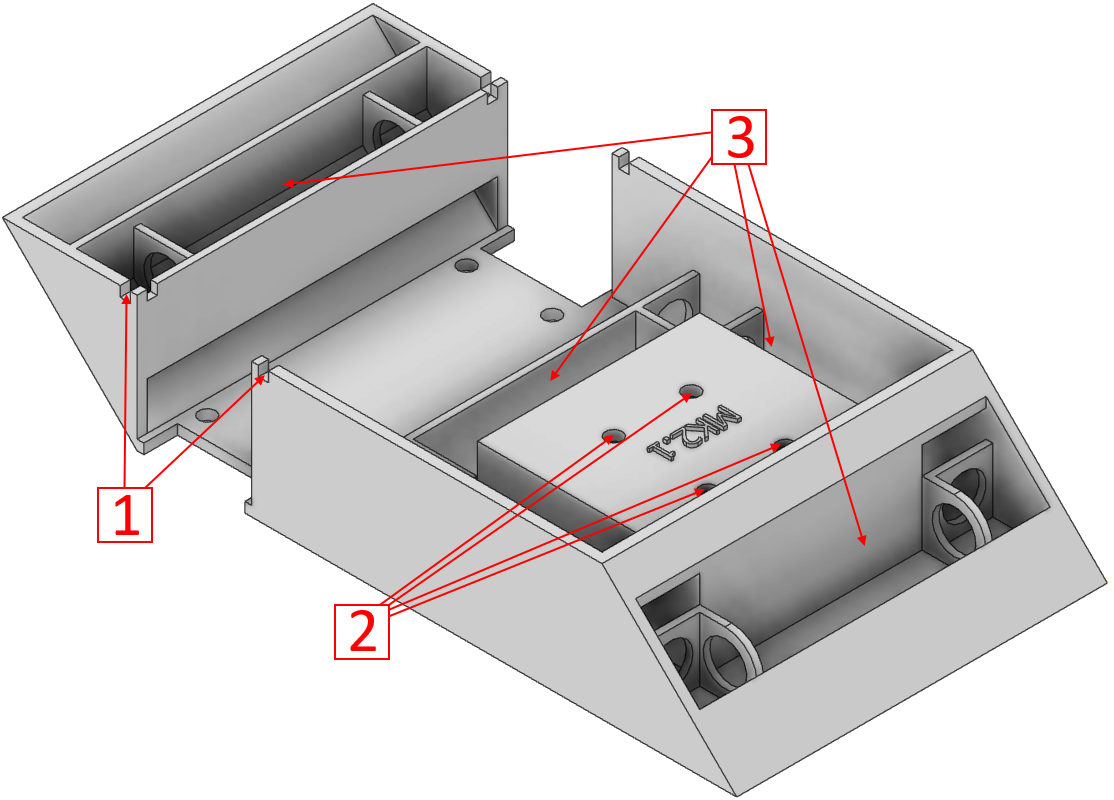
\includegraphics[scale=0.38]{images/Model3D_Rama.png}
      \label{fig:model3dramagora}
    }\qquad
    \subfloat[Widok z dołu]{
      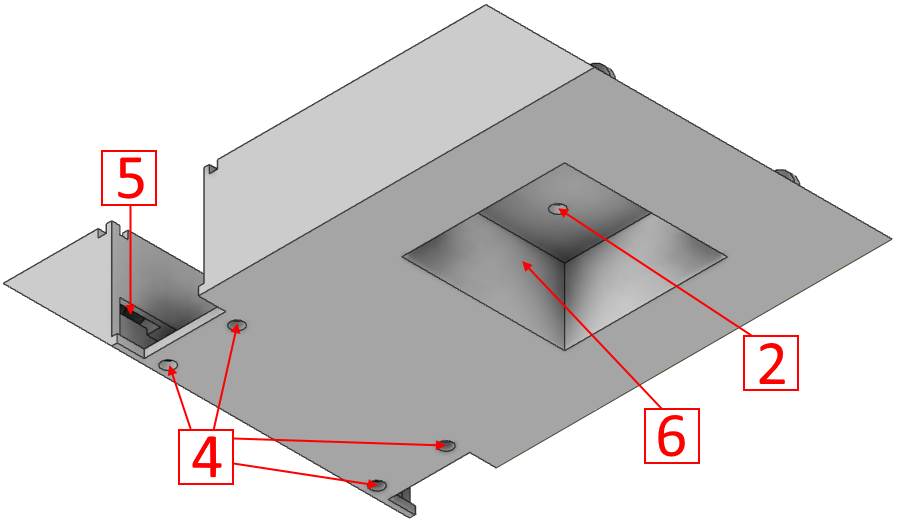
\includegraphics[scale=0.47]{images/Model3D_Rama_Spod.png}
      \label{fig:model3dramaspod}
    }
    \caption{Model 3D ramy pojazdu: a) widok z góry, b) widok z dołu}
    \label{fig:model3drama}
\end{figure}

\begin{enumerate}
    \item Uchwyty na osłony silników
    \item Otwory na śruby mocujące koło podporowe
    \item Sloty na akumulatory zasilające
    \item Otwory na śruby mocujące osłony silników
    \item Otwory na przewody akumulatorów zasilających
    \item Przestrzeń na koło podporowe
\end{enumerate}

Drugim modułem modelu 3D są osłony silników. Zakładana odległość pojazdu od ziemii wynosi 5~mm, więc wraz ze wzrostem średnicy kół konieczne jest podniesienie tylnej osi. W~przeciwnym wypadku, pojazd zacząłby podnosić się z~tylu, co spowodowałoby przy większych średnicach uderzenie przodu pojazdu o~podłoże. Model został więc stworzony tak, by zmieniać wysokość osi w razie potrzeby. Model osłony silników dla kół o~średnicy 30~mm przedstawiono na Rysunku \ref{fig:oslonasilnikow}.

\begin{figure}[!h]
    \centering
    \subfloat[Widok z góry]{
        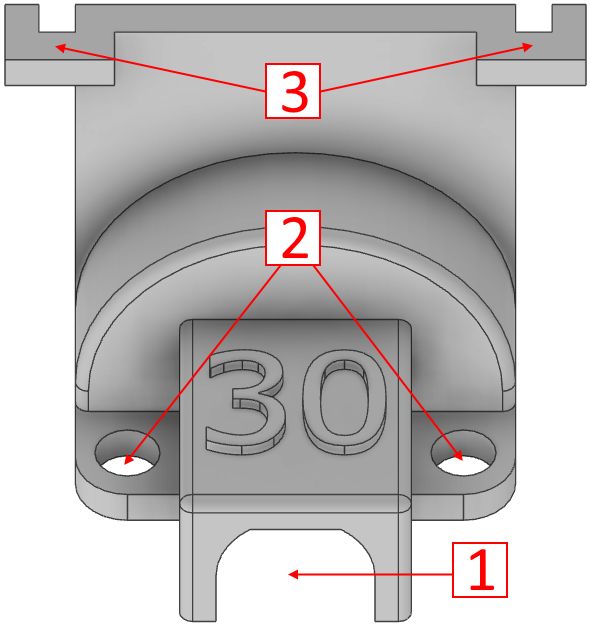
\includegraphics[scale=0.35]{images/Model3D_Oslona_1.png}
      \label{fig:moslonasilnikowgora}
    }\qquad
    \subfloat[Widok z dołu]{
      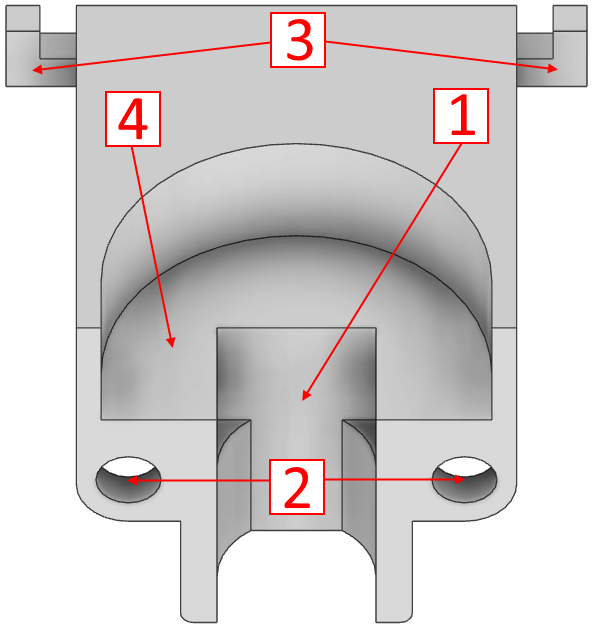
\includegraphics[scale=0.35]{images/Model3D_Oslona_2.png}
      \label{fig:oslonasilnikowspod}
    }
    \caption{Model 3D osłony silnika: a) widok z góry, b) widok z dołu}
    \label{fig:oslonasilnikow}
\end{figure}

\begin{enumerate}
    \item Przestrzeń mocowania silnika
    \item Otwory na śruby mocujące osłony silników
    \item Uchwyty przytwierdzające osłony do ramy
    \item Przestrzeń koła
\end{enumerate}

Ostatnim elementem pojazdu są koła. Podstawową wartością w~projekcie jest średnica 30~mm. Model widoczny na Rysunku \ref{fig:kolo}

\begin{figure}[!h]
    \centering
    \subfloat[Widok z góry]{
        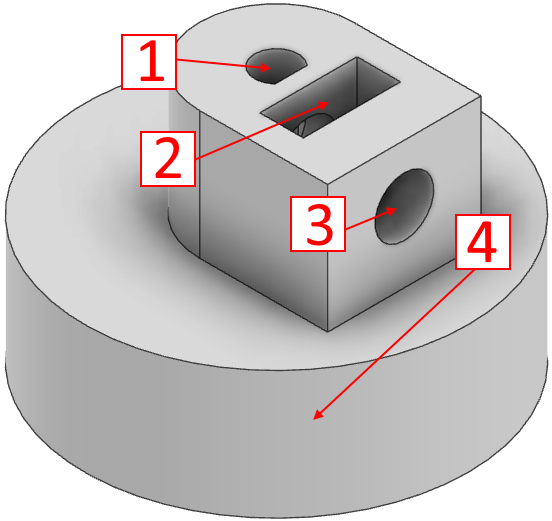
\includegraphics[scale=0.38]{images/Model3D_Kolo_1.png}
      \label{fig:kologora}
    }\qquad
    \subfloat[Widok z dołu]{
      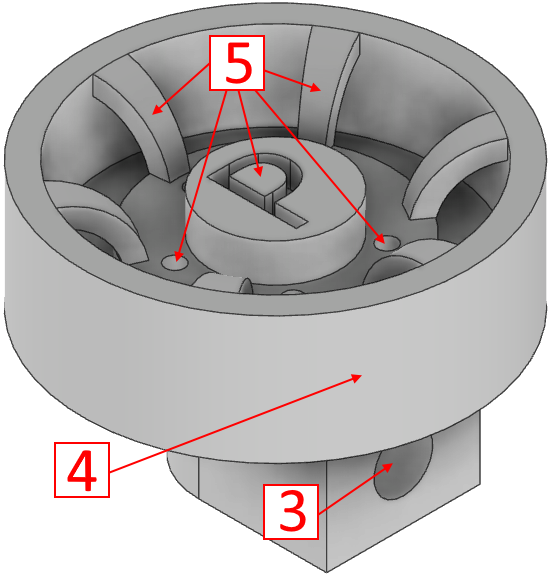
\includegraphics[scale=0.35]{images/Model3D_Kolo_2.png}
      \label{fig:kolospod}
    }
    \caption{Model 3D osłony silnika: a) widok z góry, b) widok z dołu}
    \label{fig:kolo}
\end{figure}

\begin{enumerate}
    \item Otwór wału silnika
    \item Przestrzeń nakładki śruby dociskowej
    \item Przestrzeń śruby dociskowej
    \item Koło
    \item Elementy ozdobne
\end{enumerate}

\subsection*{Elektronika}
Podstawową funkcją układu elektronicznego jest obsługa 2~silników DC. Wymaga to zastosowania elementu generującego sygnał sterujący, zasilania, oraz części przekazującej moc do silników. Jako serce układu wybrano mikrokontroler ESP32-DevKitC~V4 (Rysunek~\ref{fig:esp32}). Odpowiada on za wszystkie najważniejsze operacje: odbieranie i~wysyłanie danych po Wi-Fi, rozpoczynanie i~kończenie pomiarów, oraz generowanie sygnału sterującego. Dokładną specyfikację techniczną pominięto, ponieważ nie jest ona istotna w kontekście projektu. Została dobrana tak, by spełniała założenia projektowe (sterowanie PWM i obsługa Wi-Fi).

\begin{center}
    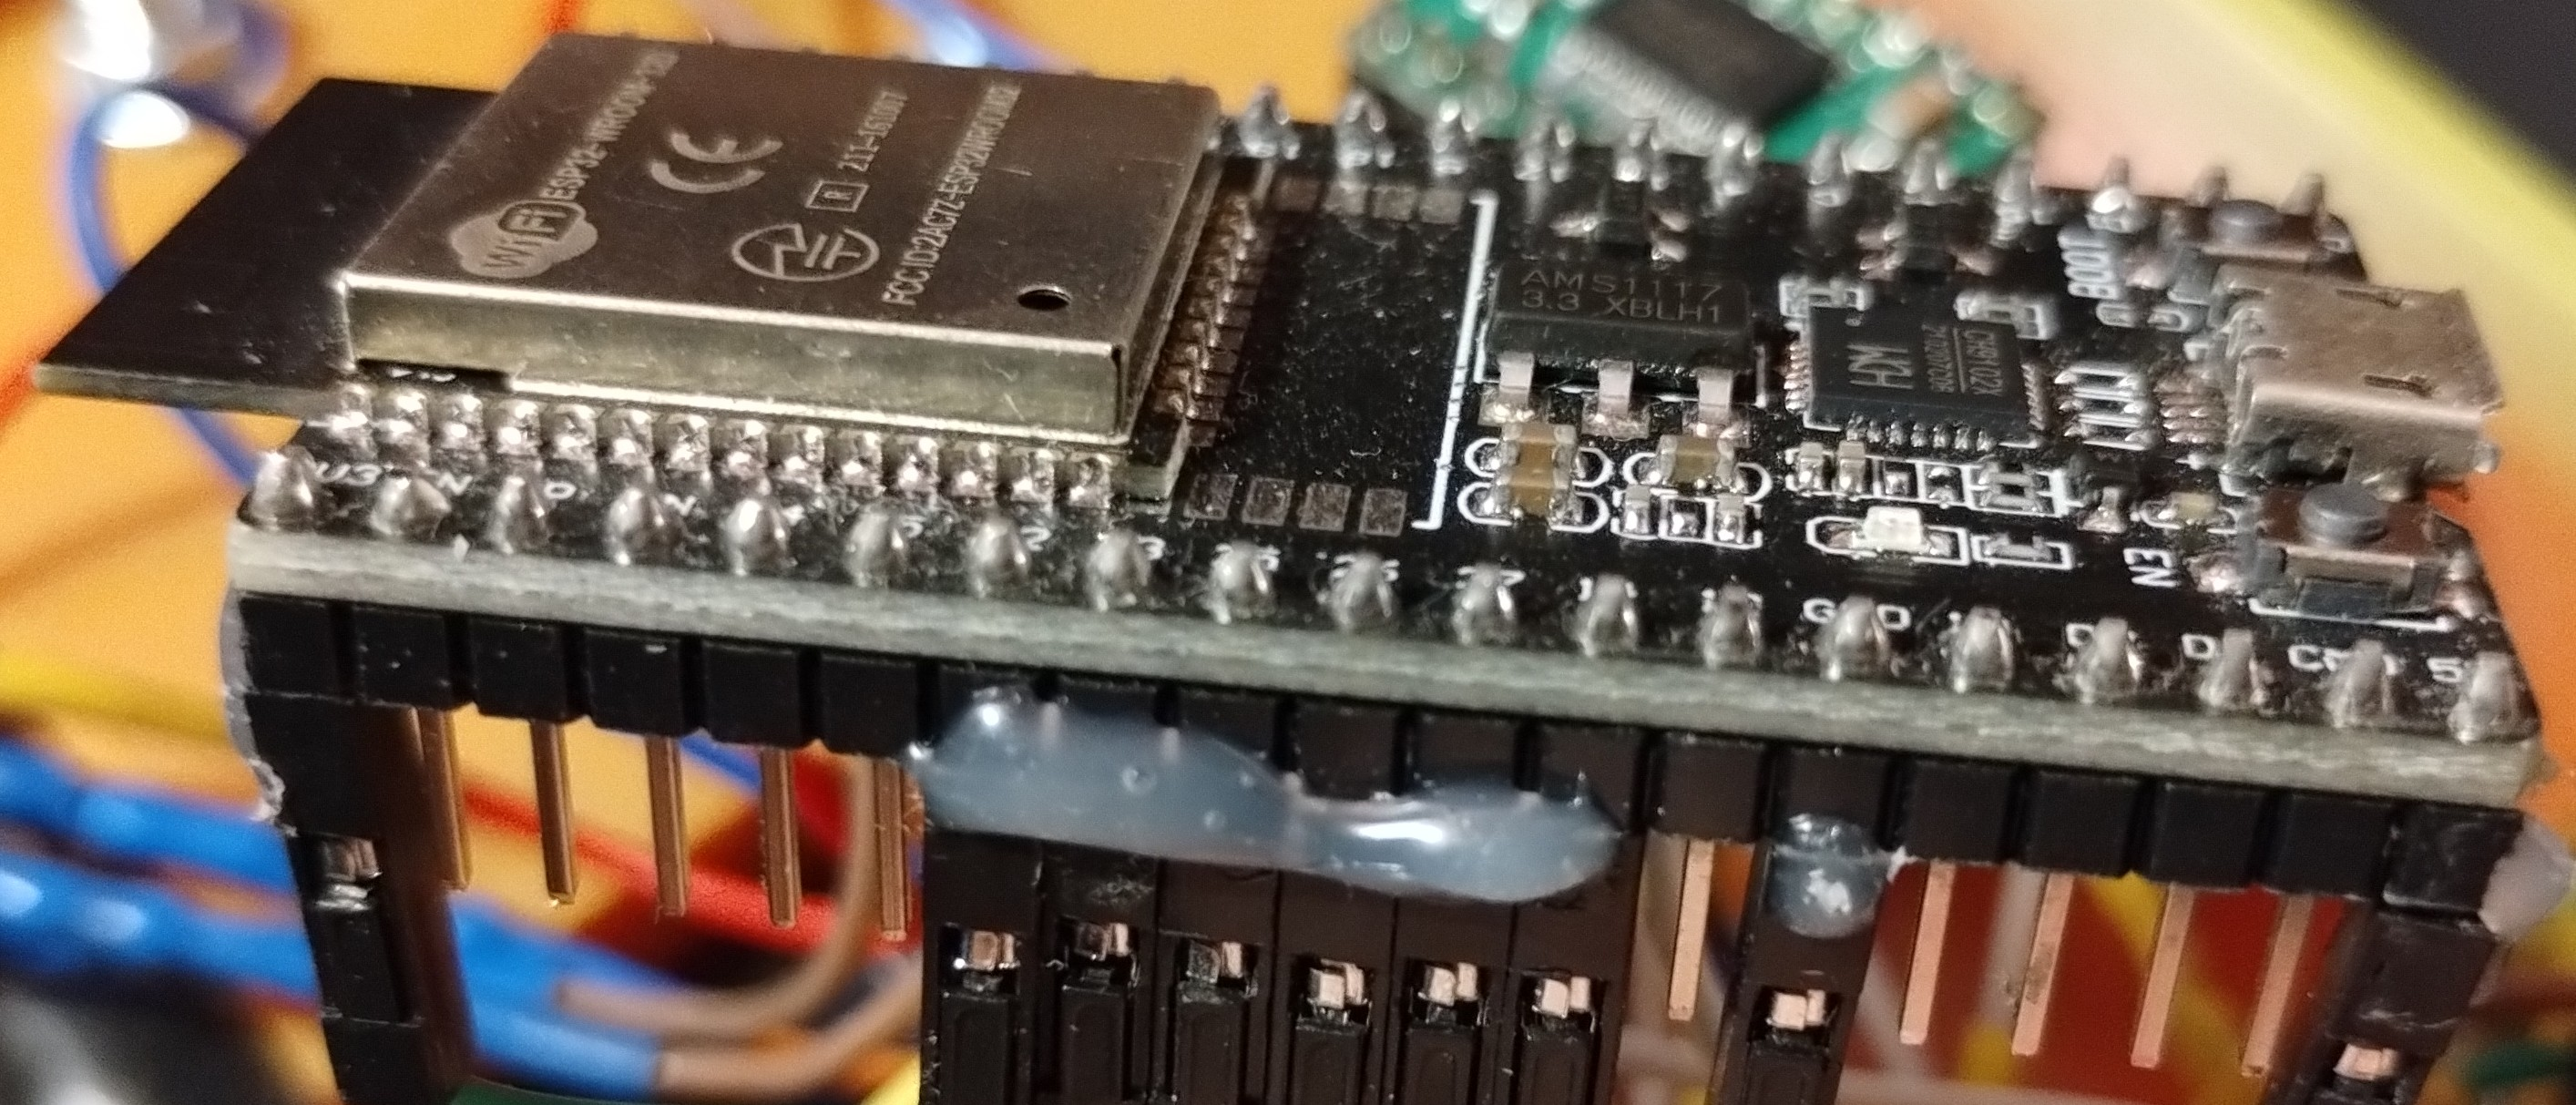
\includegraphics[scale=0.08]{images/ESP32.jpg}
    \captionof{figure}{Płytka mikrokontrolerowa ESP32-DevKitC V4}
    \label{fig:esp32}
\end{center}

Napędem są 2~silniki DC z~enkoderami magnetycznymi widoczne na Rysunku \ref{fig:motor}. Informacyjnie zamieszczono również ich specyfikację w~Tabeli \ref{tab:motor}.

\begin{center}
    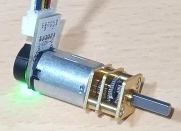
\includegraphics[scale=1]{images/Silnik.png}
    \captionof{figure}{Silnik DC z enkoderem magnetycznym (Źródło: \cite{bib:silnikali})}
    \label{fig:motor}
\end{center}

\begin{table}[!h]
    \begin{tabular}{|cccccc|}
    \hline
    \multicolumn{6}{|c|}{\textbf{Specyfikacja silników}} \\ \hline
    \multicolumn{1}{|c|}{\begin{tabular}[c]{@{}c@{}}Napięcie\\ zamionowe\end{tabular}} & \multicolumn{1}{c|}{12 V}  & \multicolumn{1}{c|}{\begin{tabular}[c]{@{}c@{}}Prędkość\\ znamionowa\end{tabular}}          & \multicolumn{1}{c|}{230 RPM}   & \multicolumn{1}{c|}{\begin{tabular}[c]{@{}c@{}}Prędkość na\\ biegu jałowym\end{tabular}}    & 300 RPM   \\ \hline
    \multicolumn{1}{|c|}{Przełożenie}                                                  & \multicolumn{1}{c|}{100:1} & \multicolumn{1}{c|}{\begin{tabular}[c]{@{}c@{}}Moment\\ obrotowy\\ znamionowy\end{tabular}} & \multicolumn{1}{c|}{200 g.cm}  & \multicolumn{1}{c|}{\begin{tabular}[c]{@{}c@{}}Moment\\ obrotowy\\ maksymalny\end{tabular}} & 1.6 kg.cm \\ \hline
    \multicolumn{1}{|c|}{\begin{tabular}[c]{@{}c@{}}Prąd\\ blokady\end{tabular}}       & \multicolumn{1}{c|}{0.9 A} & \multicolumn{1}{c|}{\begin{tabular}[c]{@{}c@{}}Prąd na\\ biegu jałowym\end{tabular}}        & \multicolumn{1}{c|}{$\leq$ 75 mA} & \multicolumn{1}{c|}{Prąd znamionowy}                                                        & $\leq$ 0.3 A \\ \hline
    \multicolumn{1}{|c|}{\begin{tabular}[c]{@{}c@{}}Liczba impulsów\\ enkodera na obrót\end{tabular}} & \multicolumn{1}{c|}{7}     & \multicolumn{1}{c|}{\begin{tabular}[c]{@{}c@{}}Napięcie\\ znamionowe\\ enkodera\end{tabular}} & \multicolumn{1}{c|}{\begin{tabular}[c]{@{}c@{}}3.3 V\\ do 5 V\end{tabular}} & \multicolumn{1}{c|}{\begin{tabular}[c]{@{}c@{}}Sygnał\\ wyjściowy\\ enkodera\end{tabular}}  & \begin{tabular}[c]{@{}c@{}}Cyfrowa\\ funkcja\\ kwadratowa\end{tabular} \\ \hline
    \end{tabular}
    \caption{Specyfikacja silnika DC z enkoderem magnetycznym (Źródło: \cite{bib:silnikali})}
\end{table}
\label{tab:motor}

Do zasilania wykorzystano akumulatory litowo-jonowe typu 18650. Ponieważ pojedynczy akumulator posiada napięcie znamionowe 3.7~V i~maksymalne 4.2~V, połączono je szeregowo w~2~grupach po 2~i~3 --- dając odpowiednio 6.4~V do 8.2~V i~10.8~V do 12.6~V --- w~celu zasilania odpowiednio ESP32 i~silników.

Zasilania nie można niestety podłączyć bezpośrednio do silników. Spowodowałoby to działanie w~trybie ciągłym na pełnej mocy, bez możliwości zmiany polaryzacji, co byłoby całkowicie sprzeczne z~założeniami projektowymi. Konieczne jest podłączenie w~taki sposób, by możliwe było przekazanie sygnału sterującego z~ESP32, oraz zmiana polaryzacji. Zastosowanie połączenia pośredniego przez samą płytkę ESP32 jest niestety niemożliwe, ponieważ nie jest w stanie ona obsłużyć tak dużych prądów. Użyto więc w~tym celu sterownika silników DC, model TB6612FNG firmy Pololu (Rysunek \ref{fig:sterownik}). Działa on na zasadzie mostka~H, umożliwiającego zmianę polaryzacji. Dzięki budowie dwukanałowej, jeden sterownik umożliwia obsługę 2~silników. Posiada również ochronę przed prądami zwrotnymi, termiczny obwód odcinający i~kondensatory filtrujące. Informacyjnie zamieszczono również jego specyfikację w~Tabeli \ref{tab:sterownik}.

\begin{center}
  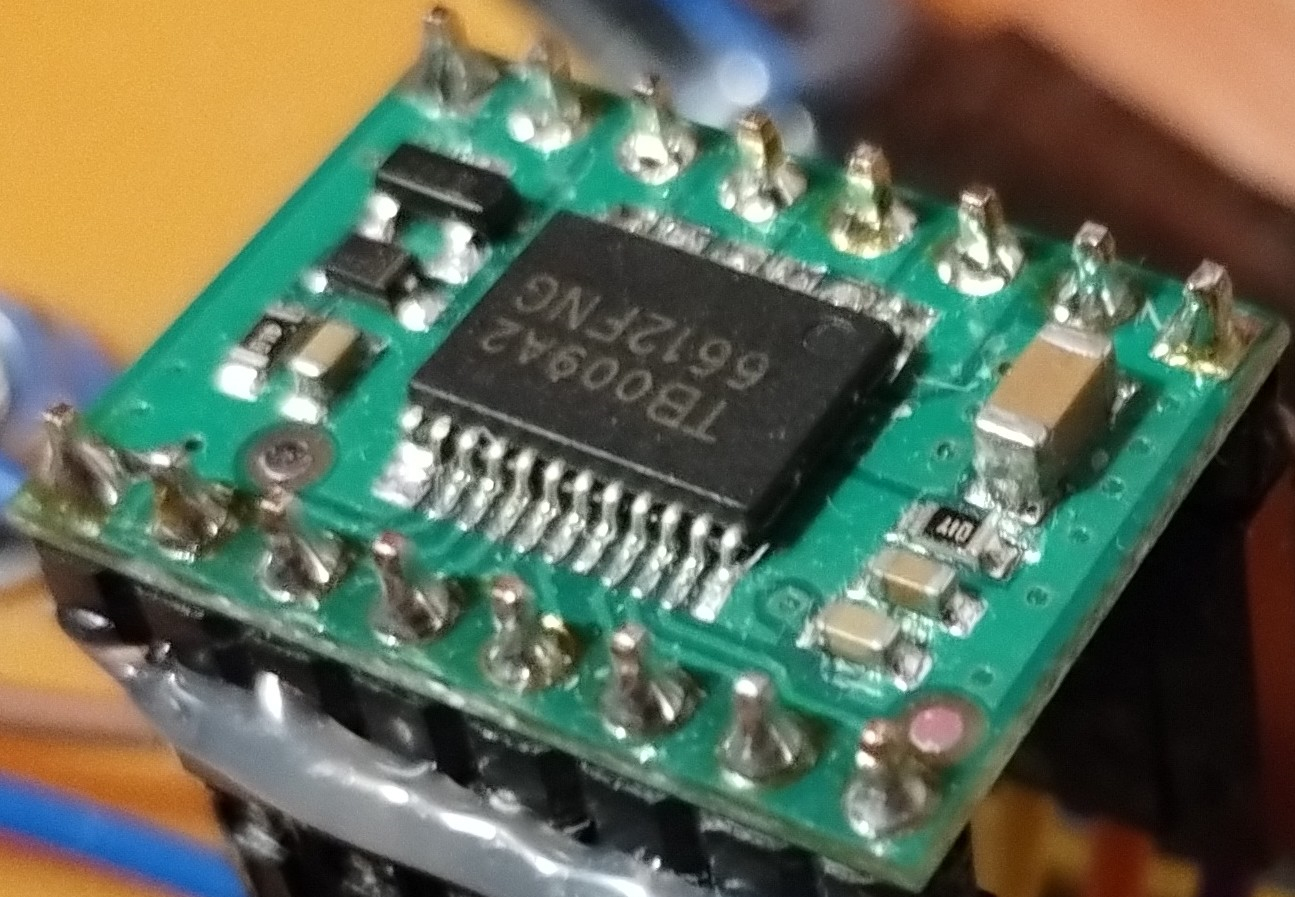
\includegraphics[scale=0.25]{images/Sterownik.jpg}
  \captionof{figure}{Sterownik silników DC TB6612FNG}
  \label{fig:sterownik}
\end{center}

\begin{table}[!h]
  \begin{tabular}{|cccccc|}
  \hline
  \multicolumn{6}{|c|}{\textbf{Specyfikacja sterownika TB6612FNG}}   \\ \hline
  \multicolumn{1}{|c|}{\begin{tabular}[c]{@{}c@{}}Zasilanie\\ silników (VMOT)\end{tabular}}        & \multicolumn{1}{c|}{\begin{tabular}[c]{@{}c@{}}4.5 V\\ do 13.5 V\end{tabular}} & \multicolumn{1}{c|}{\begin{tabular}[c]{@{}c@{}}Zasilanie układu\\ logicznego (VCC)\end{tabular}}    & \multicolumn{1}{c|}{\begin{tabular}[c]{@{}c@{}}2.7 V\\ do 5.5 V\end{tabular}} & \multicolumn{1}{c|}{\begin{tabular}[c]{@{}c@{}}Maksymalna\\ częstotliwość\\ PWM\end{tabular}} & 100 kHz \\ \hline
  \multicolumn{1}{|c|}{\begin{tabular}[c]{@{}c@{}}Ciągły prąd\\ wyjściowy\\ na kanał\end{tabular}} & \multicolumn{1}{c|}{1 A}                                                       & \multicolumn{1}{c|}{\begin{tabular}[c]{@{}c@{}}Maksymalny\\ prąd wyjściowy\\ na kanał\end{tabular}} & \multicolumn{1}{c|}{3 A}                                                      & \multicolumn{1}{c|}{\begin{tabular}[c]{@{}c@{}}Łączny ciągły\\ prąd maksymalny\end{tabular}}  & 2 A     \\ \hline
  \end{tabular}
  \caption{Specyfikacja sterownika silników DC TB6612FNG (Źródło: \cite{bib:sterownik})}
\end{table}
\label{tab:sterownik}

Dużym wyzwaniem okazał się dobór odpowiedniego czujnika laserowego, który z~wysoką precyzją mierzyłby dokładność przebytej odległości i~pomiarów z enkoderów. Pierwszym problemem był wybór takiego czujnika, który działałby z~odpowiednią precyzją i~dokładnością. Wymagana jest dokładność poniżej 5~mm, idealnie w~okolicach 1~mm. Drugi problem to kąt działania czujnika. Większość z~nich oferuje kąt działania w~okolicach 15$^{\circ}$ symetryczny wokół środka, dając promień 7.5$^{\circ}$. Czujnik znajdowałby się bardzo blisko podłogi, co tworzyłoby ryzyko, że utworzony przez kąt działania stożek uderzałby o~podłogę i~wykrywał ją jako przeszkodę, lub wykrywał inne niepożądane poboczne obiekty, niwelując tym samym użyteczność otrzymanych pomiarów. Dalmierze oferujące pomiar punktowy lub bliski punktowemu posiadają znaczne wymiary, niską kompatybilność z~elektroniką hobbystyczną (ESP32), dużą masę, i/lub wysoką cenę. Rozwiązaniem alternatywnym byłoby wykorzystanie systemu LIDAR (ang.~\english{Light Detection and Ranging}), który umożliwia nie tylko punktowy pomiar odległości, lecz mapowanie danego obszaru wykorzystując technologię czujników laserowych. Istnieją modele spełniające założenia projektowe i~mieszczące się w sensownym budżecie, jednak ich wykorzystanie wymagałoby znacznych nakładów czasowych w~celu nauki sprzętu, zaprogramowania odpowiednich funkcjonalności, a~następnie testów. Z~tego powodu zdecydowano o~porzuceniu idei pomiaru laserowego i~zamiast tego wykorzystanie pomiaru manualnego z~pomocą dostępnego powszechnie przymiaru liniowego.

Enkodery magnetyczne zostały zapewnione w~silnikach napędowych --- stanowią wspólną całość, wymagane jest jedynie ich odpowiednie podłączenie w postaci przewodów zasilających i~sygnałowych. Schemat widoczny na Rysunku \ref{fig:schematelektryczny}.

Do sygnalizowania stanu oprogramowania ESP32, czyli aktualnego stanu w jakim znajduje się układ, założono instalację LED oraz głośnika. Po zamontowaniu LED w układzie i przetestowaniu rozwiązania, okazało się, że jest ono wystarczające do spełnienia założonego celu. Tym samym, montaż głośnika stał się zbędny i usunięto go z założeń projektowych.



\subsection*{Oprogramowanie}


\section{Narzędzia pomocnicze}

\subsection*{Skrypt MATLAB}

\subsection*{Skrypt Python}

\subsection*{Aplikacja}